\subsection{Tempo di esecuzione}

Nel calcolare il tempo di esecuzione di un algoritmo parallelo, la grandezza nota come complessità di tempo (utile nell'analisi del tempo di esecuzione di un algoritmo sequenziale) risulta poco indicativa.\\
Infatti, in un algoritmo parallelo il numero delle operazioni non coincide più con il numero dei passi temporali. Di conseguenza si introducono nuove grandezze al fine di realizzare un'analisi degli algoritmi paralleli.

Adattando i concetti del calcolo parallelo in calcolatori MIMD a memoria distribuita a quelli a memoria condivisa: se $T$ che indica il numero di thread eseguibili parallelamente dai core della macchina, un problema che si risolve in un tempo $t$ verrà risolto da $T$ thread (idealmente) in $\frac{t}{T}$.

\subsection{Speed-up, Overhead ed Efficienza}

Lo \textbf{speed-up} misura la riduzione del tempo di esecuzione rispetto all'algoritmo sequenziale ed è definito dal rapporto:
$$ S(T) = \frac{t(1)}{t(T)} $$ 

La quantità che misura quanto il nostro speed up differisce da quello ideale è l'overhead. Si può quantificare con la seguente formula: $O_h(T) = T\cdot t(T) - t(1)$ .\\
Riscrivendo lo speed up in funzione dell'overhead ci accogiamo infatti che lo speed up è ideale se e solo se l'overhead è nullo.\\

Per poter misurare se e quanto è stato "sfruttato" il nostro ambiente di calcolo parallelo, si introduce l' \underline{efficienza} del nostro algoritmo.
Si definisce \textbf{efficienza} il rapporto: $$ E(T) = \frac{S(T)}{T} $$

\subsection{Modifiche al codice per la registrazione dei tempi}
\subsubsection{Header file}
Il linguaggio C fornisce un tipo built-in per gestire la grandezza fisica del tempo: $time$.
La sua definizione é contenuta nel file header che segue e che pertanto deve essere incluso nel codice sorgente:
\begin{lstlisting}
#include <sys/time.h>
\end{lstlisting}

\subsubsection{Main}
Il main delega il calcolo dell'effettivo algoritmo all'algoritmo stesso, passando la variabile time alla funzione $matrixVector$.
La variabile $numThreads$ é invece un discriminante per l'analisi finale dei dati.
Sia time che numThreads verranno modificate a runtime dalla funzione $matrixVector$.
Infine, invochiamo $writeResultOnFile$ per registrare il risultato ottenuto.
\begin{lstlisting}
    int main(){
        double time;
        int numThreads;

        int m, n;
        double **A = readMatrixFromFile("<path>", &m, &n);
    
        int dim;
        double *x = readVector("<path>", &dim);
    
        if(dim != n){
            printf("Vettore e matrice non hanno dimensioni adeguate per una moltiplicazione...");
            exit(-1);
        }
        
        double *y = matrixVector(m, n, x, A, &time, &numThreads);
        printVector(y, m);
        writeResultOnFile("results.txt", m, n, time, numThreads);
        printf("execution time--->%.10lf", time);
    
        return 0;
    }
\end{lstlisting}

\subsection{Algoritmo}

La variabile numThreads viene inizializzata con il valore restituito dalla funzione $omp\_get\_max\_threads()$, una funzione della libreria omp che restituisce il massimo numero di thread disponibili per la successiva regione parallela.
Ai fini del calcolo del tempo d'esecuzione, ci serviamo della funzione $gettimeofday$, che restituisce un oggetto di tipo struct timeval, contenente il clock, il giorno di sistema ed altre informazioni.
Alla prima chiamata a $gettimeofday$, salviamo il valore in secondi nella variabile $timeStart$, mentre alla seconda, salviamo in $timeEnd$.
L'istruzione che inizializza la variabile $timeStart$ somma i secondi conservati da t ai microsecondi conservati da t divisi per 1000000 (i microsecondi vengono riscalati a secondi).
Assegniamo al parametro time il la differenza tra $timeEnd$ e $timeStart$.
\begin{lstlisting}
    double *matrixVector(int m, int n, double *x, double **A, double *time, int *numThreads){
        (*numThreads) = omp_get_max_threads();
    
        struct timeval t;
        gettimeofday(&t, NULL);
        double timeStart = t.tv_sec+(t.tv_usec / 1000000.0);

        double *y = calloc(m, sizeof(double));
        int i, j;
        #pragma omp parallel for default(none) shared(m,n,x,A,y) private(i,j)
            for (i = 0; i < m; i++){
                for (j = 0; j < n; j++){
                    y[i] += A[i][j] * x[j];
                }
            }

        gettimeofday(&t, NULL);
        double timeEnd = t.tv_sec+(t.tv_usec / 1000000.0);

        (*time) = timeEnd - timeStart;

        return y;
    }
\end{lstlisting}

\subsubsection{Scrittura dei tempi raccolti}
Segue la definizione della funzione invocata alla fine del main: writeResultOnFile.
\begin{lstlisting}
    void writeResultOnFile(char *path, int m, int n, double time, int numThreads){
        FILE *fp;
        fp = fopen(path,"a");

        fprintf(fp, "Dimensione in Input: %dx%d \nTempo di esecuzione: (%.10lf secondi) \nNumero di thread nel team: %d\n\n\n", m, n, time, numThreads);
        fclose(fp);
    }
\end{lstlisting}

\subsection{Dati empirici}
L'algoritmo è stato testato in più condizioni e secondo i parametri precedentemente descritti.
É stato fissata una dimensione di 10000x10000 per la matrice in input e di 1000 per il vettore.
Il numero di thread é variato da 1 a 8, tenendo conto delle sole potenze di 2.

\begin{table}[htp]
\centering
%\caption{}
\begin{tblr}{
  hlines,
  vlines,
}
Threads & Tempo ($\cdot 10^{-1} s$) & Speed Up & Efficienza & Overhead ($\cdot 10^{-1} s$) \\
1          & 9.606   & x    & x       & x                     \\
2          & 4.859   & 1.977    & 0.988       & 0.12                     \\
4          & 2.506   & 3.83    & 0.957       & 0.14                     \\
8          & 1.402   & 6.851    & 0.856       & 1.61                     \\
16         & 1.562   & -    & -       & -
\end{tblr}
\end{table}


\clearpage

Il grafico dei tempi:
\begin{figure}[h!tbp]
    \centering
    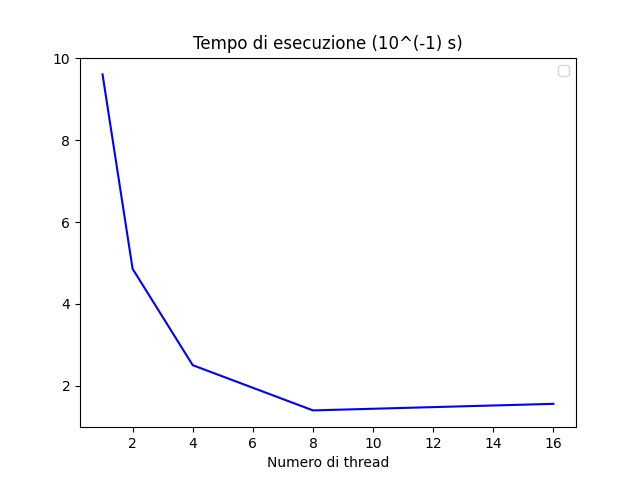
\includegraphics[width=1\linewidth]{tempi.png}
    \caption{Andamento dei tempi}
    \label{fig:enter-label}
\end{figure}
Si noti come, con 16 thread, il tempo sia peggiorato. Questo è stato previsto poiché la macchina su cui si è effettuato il test poteva eseguire al più 8 thread contemporaneamente. Eseguirne più di 8 ha causato quindi un collo di bottiglia.

\newpage
Visualizziamo la curva, confrontandola all'andamento dello speed-up ideale:
\begin{figure}[h!tbp]
    \centering
    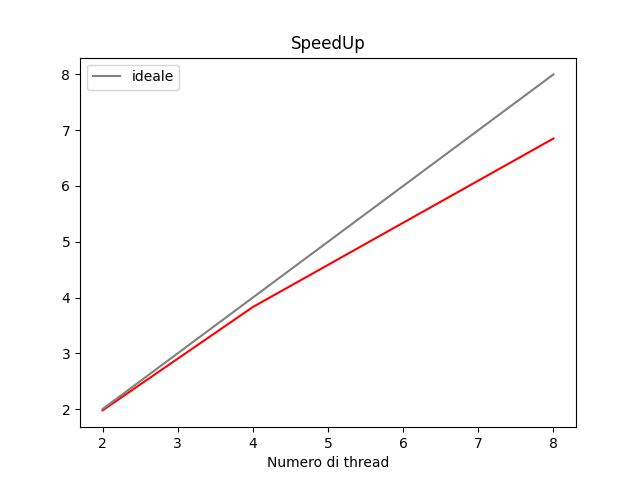
\includegraphics[width=1\linewidth]{speedup.png}
    \caption{Andamento dello Speed Up}
    \label{fig:enter-label}
\end{figure}
\clearpage
Visualizziamo su un grafico anche i valori dell'Overhead:

\begin{figure}[h!tbp]
    \centering
    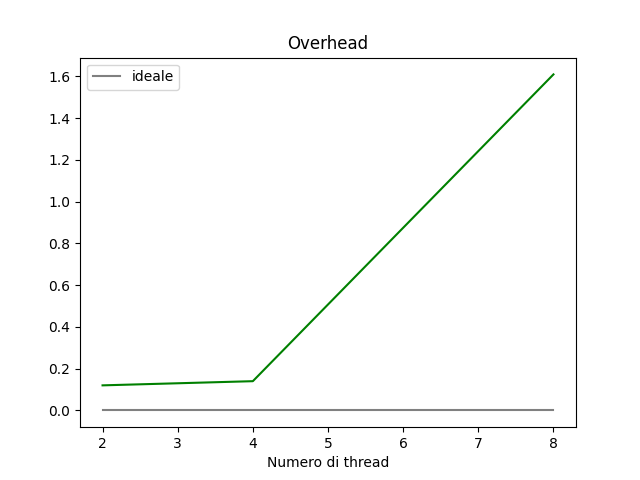
\includegraphics[width=1\linewidth]{overhead.png}
    \caption{Andamento dell'Overhead}
    \label{fig:enter-label}
\end{figure}

\clearpage

Infine osserviamo come varia la nostra efficienza:
\begin{figure}[h!tbp]
    \centering
    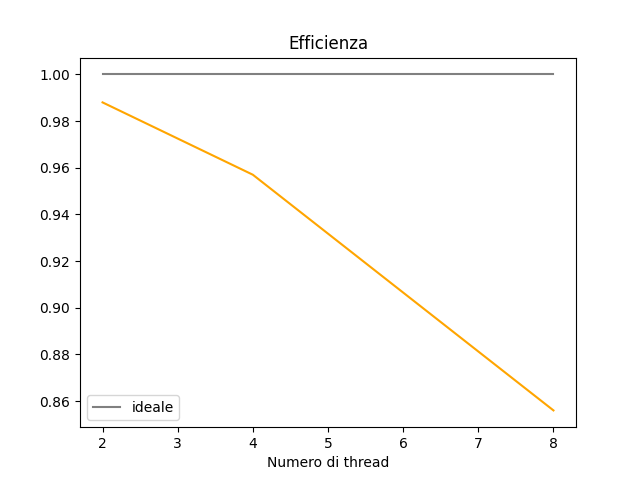
\includegraphics[width=1\linewidth]{efficienza.png}
    \caption{Andamento dell'efficienza}
    \label{fig:enter-label}
\end{figure}